\paragraph{Существующие подходы}

\begin{itemize}
    \item {
        Visibility culling (Отбор видимых полигонов).

        Visibility culling~--~это семейство алгоритмов,
        нацеленное на предотвращение вызовов отрисовки
        для объектов невидимых в кадре.%
        \cite{Cohenor2002}
        Пример различных техник отбора видимых полигонов
        показан на рисунке~\ref{figure:CullingTechniques}.
        Подобные алгоритмы являются очень эффективными,
        когда количество объектов единовременно видимых в виртуальной сцене
        значительно меньше их общего количества,
        например в замкнутых помещениях внутри крупного здания.

        \begin{figure}[!htp]
            \centering
            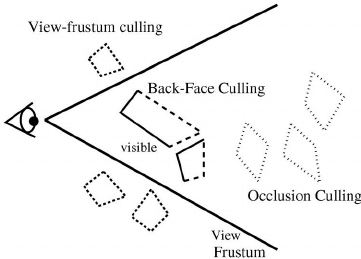
\includegraphics[width=0.8\textwidth]
            {images/Three-types-of-visibility-culling-techniques.png}
            \caption{Техники отбора видимых полигонов.%
            \cite{Cohenor2002}}
            \label{figure:CullingTechniques}
        \end{figure}

        \begin{itemize}
            \item {
                View-frustum culling~--~это техника отбора,
                отсекающая отрисовку объектов,
                находящихся за границами поля зрения виртуальной камеры.
            }
            \item {
                Back-face culling~--~это техника отбора,
                позволяющая избежать отрисовку геометрии,
                направленной в противоположную сторону от виртуальной камеры.
            }
            \item {
                Occlusion culling~--~это техника отбора,
                предотвращающая отрисовку геометрии,
                скрытой за другими объектами виртуальной сцены.
            }
        \end{itemize}
    }
    \item {
        LOD (англ. Level of detail~--~уровень детализации).

        LOD~--~это оптимизационная техника,
        нацеленная на снижение используемого количества
        полигонов модели при ее удалении от виртуальной камеры.
        Для работы метода требуется создать несколько версий
        одной и той же модели с разным уровнем детализации (количеством полигонов),
        как это показано на рисунке~\ref{figure:LOD0-1}.

        \begin{figure}[!htp]
            \centering
            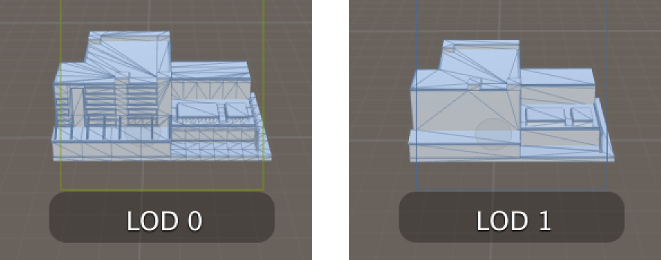
\includegraphics[width=0.8\textwidth]{images/LOD0-1.png}
            \caption{Разные уровни детализации.%
            \cite{DocUnity}}
            \label{figure:LOD0-1}
        \end{figure}

        Перед вызовом запроса отрисовки производится выбор необходимой модели,
        то есть вблизи от виртуальной камеры будут отрисовываться
        детализированные модели (LOD0), а вдали упрощенные (LOD1-LOD3).
    }
    \item {
        Batching.

        Батчинг~--~это оптимизационная техника,
        предназначенная для снижения количества запросов отрисовки
        за счет группировки нескольких полигональных сеток.

        \begin{itemize}
            \item {
                Батчинг может происходить динамически, если
                группируется множество простых объектов,
                с одинаковыми графическими материалами и текстурами
                (чего можно добиться с помощью создания атласа текстур).
                За счет этого можно отрисовывать несколько движущихся объектов
                за один вызов отрисовки, что имеет смысл, если продолжительность
                группировки меньше, чем затраты на многочисленные вызовы отрисовки.
            }
            \item {
                С другой стороны батчинг может быть статическим, то есть
                происходить однократно и объединять неизменяемую геометрию
                в одну полигональную сетку, позволяя достичь ещё большей производительности,
                чем при динамической группировке.
                Стоит отметить, что подобная группировка снижается
                эффективность отбора видимых полигонов, так как
                сгруппированные объекты начнут восприниматься как один.
            }
        \end{itemize}
    }
    \item {
        Geometry instancing (Дублирование геометрии).

        Geometry instancing~--~это методика, позволяющая
        одновременно рендерить нес\-колько объектов, имеющих
        одинаковую полигональную сетку.
        Такой подход в основном используется для отрисовки
        повторяющихся фоновых объектов, таких как растительность или здания.
        Объекты могут иметь разное положение в пространстве,
        размеры, отличающиеся графические материалы.
        Дублирование геометрии значительно снижает
        количество запросов на отрисовку.
    }
\end{itemize}
